%\subsubsection{Illustrative example}
%\label{sec:illustrative example}
\begin{exmp}
We consider a linear system with the following dynamics:
\begin{equation}
\label{eq:PointMass}
x_{k+1} = x_k + u_k
\end{equation}

The specification is 
\[\formula = \always_{[0,20]} \neg (x \in \text{Unsafe}) \land \eventually_{[0,20]} (x \in \text{Terminal})\]
with the sets $\text{Unsafe}=[-1,1]^2$ and $\text{Terminal}=[2,2.5]^2$. 
The state space is $X=[-2.5,2.5]^2$, $U=[0.3,0.3]^2$, $\delta=1$, and we optimize for two different values of $\gamma$, $0.1$ and $0.001$. 
The initial point of the trajectory is $x_0=[-2,-2]'$. 
The control cost is $l(x_k,u_k) = ||x_k||_{2}^2$, so that longer trajectories incur greater cost. 
Finally, $hrz(\formula) = 21$.

\textbf{Results}.
Fig. \ref{fig:toy control} shows the found trajectories from the two methods in modes (B) and (R), starting from the same initial state. 
All experiments use $\gamma=0$ except that last one
\todo[inline]{fix BluSTLS in figure}
Both BluSTL (B) and SR-SQP (B) produce satisfying trajectories.

Note that BluSTL results in a trajectory that skirts the edge of the unsafe set and reaches a corner of the terminal set (resulting robustness is zero). SR-SQP (B) and SR-SQP (R) have a similar shape but SR-SQP (R) ends in the middle of the terminal set, resulting in a higher robustness as expected, while SR-SQP (B) terminates on reaching a positive robustness threshold as described above. SR-SQP (R,$\gamma=0.1$), takes into account the control cost and hence results in a trajectory of shorter length which trades of robustness ($0.236$ compared to $0.247$ for SR-SQP (R)) for control cost as is expected from the objective of $P_{\srob}$ in Eq. \ref{eq:general_ctrl}.
The last trajectory corresponds to SR-SQP in \textit{robust} mode with a non-zero cost for control corresponding to $\gamma=0.1$  in $P_{\srob}$ and a quadratic control cost function $l$. 

For detailed evaluation, we run 100 instances with the specification and dynamics of our illustrative example, with a random initial state $x_0 \in [-2.5,-1.5] \times [-2.5,2.5]$ for each instance. We also vary the formula horizon (and hence optimization length of the trajectory being optimized over) $N$ from $20$ to $200$ time-steps. Table \ref{tbl:time_performance_toy} shows the execution times for each method and the two modes of operation. All experiments were run on a machine with a quad-core Intel I5 3.2GHz processor with 24GB RAM, running MATLAB 2016b.


\begin{table}[tb]
\small
\begin{center}
\caption{{\small Runtimes (mean and standard, in seconds) for Smooth Operator (SR-SQP) and BluSTL (BlS) over 100 runs with random initial states and with different formula horizon lengths $N$. Here, (B) means \textit{boolean} mode and (R) means \textit{robust} mode of operation.}}
\vspace{-5pt}
\label{tbl:time_performance_toy}
\begin{tabular} {|c|c|c|c|c|}
	\hline
	N & BlS(B) & SR-SQP(B) & BlS(R) & SR-SQP(R) \\ \hline
	20 & $0.96 \pm 0.82$ &  $\mathbf{0.31 \pm 0.13}$  & NA & $3.30 \pm 1.25$ \\ \hline
	30 & $1.37 \pm 1.72$ &  $\mathbf{0.33 \pm 0.25}$  & NA & $5.85 \pm 2.74$\\ \hline
	40 & $3.86 \pm 5.10$ &  $\mathbf{0.60 \pm 0.29}$  & NA & $12.36 \pm 6.04$\\ \hline
	50 & $4.36 \pm 12.97$&  $\mathbf{0.74 \pm 0.30}$ & NA & $30.05 \pm 18.23$\\ \hline
	100& $16.77 \pm 27.84$ & $\mathbf{1.21 \pm 0.25}$ & NA & $69.70 \pm 13.16$ \\ \hline
	200& $53.88 \pm 14.18$& $\mathbf{4.19 \pm 1.18}$ & NA & $126.11 \pm 20.43$ \\ \hline
\end{tabular}	
\end{center}
\end{table}

\textbf{Analysis.}
As seen in table \ref{tbl:time_performance_toy}, our method is consistently faster than BluSTL for the \textit{boolean} mode, and also displays smaller variances in runtimes. For BluSTL in \textit{robust} mode, BluSTL could not finish a single instance of robustness maximization within 100 hours on both the machine used for running experiments as well as on a machine with 8 core Intel Xeon machine with 60GB RAM, leading us to believe that the problem formulation in BluSTL did not scale into a tractable MILP. Note, the problem solved here is very similar to the example used in \cite{Saha_acc16}, which uses another MILP based method to find satisfying trajectories. While the underlying dynamics and the machine on which evaluations are run are different, these results suggest that our run-times compare favourably with those in \cite{Saha_acc16}.

When in \textit{boolean} mode, BluSTL results in trajectories with zero robustness (as seen in fig. \ref{fig:toy control}), while our method results in trajectories with an average robustness of 0.10. Both methods satisfy $\formula$ in all 100 instances. In \textit{robust} mode, across all experiments, SR-SQP results in an average $\rob_{\formula}=0.247$ with a standard deviation of less than $0.005$. It is to be noted, that an upper bound on the maximum achievable $\rob_{\formula}$ is $0.25$, which can be achieved by trajectory reaching (in number of time steps $\leq N$) the point $[2.25,2.25]$ in the middle of the Terminal set while always avoiding the Unsafe set by a distance greater than $0.25$. This shows that for this problem, our method reaches very close to achieving the global optima of $\rob_{\formula}$. Also with this additional knowledge of the global optima upper bound, the SR-SQP method in \textit{robust} mode can be made a lot faster by specifying an exit condition based on a upper threshold of $\srob_{\formula}$ attained at any iteration of the SR-SQP method. While for brevity we do not include results with this additional stopping criteria, it was observed that for an upper bound value of $\srob_{\formula}=0.24$, an average speed up of about $4$-times was observed for $N=20$ and $2$-times for $N=200$ while resulting an average robustness value achieved of $\rob_{\formula} = 0.235$. This shows that with the iterative nature of SQP, we can trade-off performance for improved execution times.

\textbf{Note} that in BluSTL, atomic propositions in general have to be of the form $a'x\leq b$ (although absolute value and polynomials are also valid) since robustness is encoded as a MILP, which necessitates avoiding the signed distance function in dimensions greater than 1. This implies that atomic propositions in higher dimensions ($x\in \mathbb{R}^{n>1}$), $Hx \leq g$, have to be broken down into the conjunction of $n$ individual atomic propositions of the form $h_i'x \leq g_i$. This also restricts atomic propositions in BluSTL from involving sets like circles or ellipsoids. On the other hand, atomic propositions in our work can involve non-Polyhedron sets (e.g. ellipsoids or circles) and even non-convex sets since we do not avoid the signed distance function for higher dimensions.

\begin{figure}[t]
\centering
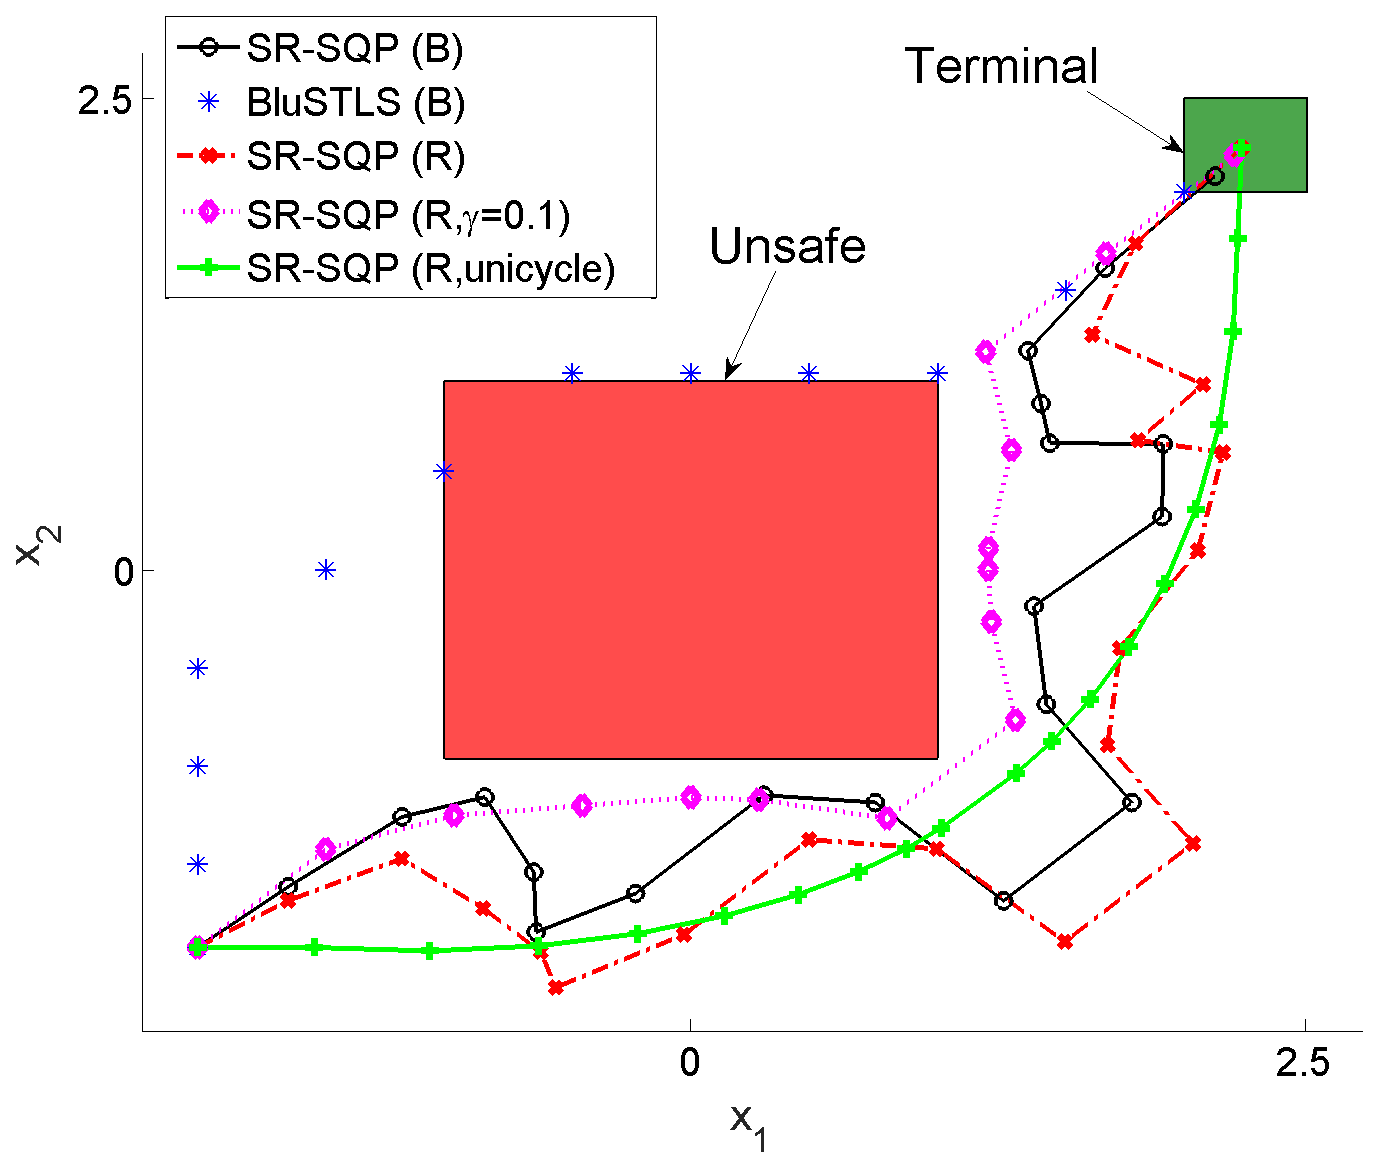
\includegraphics[width=0.49\textwidth]{figures/ToyExUni_scissored.pdf}
\vspace{-20pt}
\caption{{\small Trajectories for the illustrative example for SR-SQP and BluSTL. B, R refer to the \textit{Boolean} and \textit{Robust} mode of operation. Refer to the discussion in Sec. \ref{sec:illustrative example}}, Results for an explanation. Color in online version.}
\label{fig:toy control}
\vspace{-10pt}
\end{figure}

\end{exmp}